% Options for packages loaded elsewhere
\PassOptionsToPackage{unicode}{hyperref}
\PassOptionsToPackage{hyphens}{url}
%
\documentclass[
  12pt,
]{article}
\usepackage{amsmath,amssymb}
\usepackage{lmodern}
\usepackage{ifxetex,ifluatex}
\ifnum 0\ifxetex 1\fi\ifluatex 1\fi=0 % if pdftex
  \usepackage[T1]{fontenc}
  \usepackage[utf8]{inputenc}
  \usepackage{textcomp} % provide euro and other symbols
\else % if luatex or xetex
  \usepackage{unicode-math}
  \defaultfontfeatures{Scale=MatchLowercase}
  \defaultfontfeatures[\rmfamily]{Ligatures=TeX,Scale=1}
  \setmainfont[]{Times New Roman}
\fi
% Use upquote if available, for straight quotes in verbatim environments
\IfFileExists{upquote.sty}{\usepackage{upquote}}{}
\IfFileExists{microtype.sty}{% use microtype if available
  \usepackage[]{microtype}
  \UseMicrotypeSet[protrusion]{basicmath} % disable protrusion for tt fonts
}{}
\makeatletter
\@ifundefined{KOMAClassName}{% if non-KOMA class
  \IfFileExists{parskip.sty}{%
    \usepackage{parskip}
  }{% else
    \setlength{\parindent}{0pt}
    \setlength{\parskip}{6pt plus 2pt minus 1pt}}
}{% if KOMA class
  \KOMAoptions{parskip=half}}
\makeatother
\usepackage{xcolor}
\IfFileExists{xurl.sty}{\usepackage{xurl}}{} % add URL line breaks if available
\IfFileExists{bookmark.sty}{\usepackage{bookmark}}{\usepackage{hyperref}}
\hypersetup{
  pdftitle={Dall sheep reproductive success in Alaska and NW Canada},
  pdfauthor={Marisa Fajardo, Clara Fast, and Julia Plasynski},
  hidelinks,
  pdfcreator={LaTeX via pandoc}}
\urlstyle{same} % disable monospaced font for URLs
\usepackage[margin=2.54cm]{geometry}
\usepackage{longtable,booktabs,array}
\usepackage{calc} % for calculating minipage widths
% Correct order of tables after \paragraph or \subparagraph
\usepackage{etoolbox}
\makeatletter
\patchcmd\longtable{\par}{\if@noskipsec\mbox{}\fi\par}{}{}
\makeatother
% Allow footnotes in longtable head/foot
\IfFileExists{footnotehyper.sty}{\usepackage{footnotehyper}}{\usepackage{footnote}}
\makesavenoteenv{longtable}
\usepackage{graphicx}
\makeatletter
\def\maxwidth{\ifdim\Gin@nat@width>\linewidth\linewidth\else\Gin@nat@width\fi}
\def\maxheight{\ifdim\Gin@nat@height>\textheight\textheight\else\Gin@nat@height\fi}
\makeatother
% Scale images if necessary, so that they will not overflow the page
% margins by default, and it is still possible to overwrite the defaults
% using explicit options in \includegraphics[width, height, ...]{}
\setkeys{Gin}{width=\maxwidth,height=\maxheight,keepaspectratio}
% Set default figure placement to htbp
\makeatletter
\def\fps@figure{htbp}
\makeatother
\setlength{\emergencystretch}{3em} % prevent overfull lines
\providecommand{\tightlist}{%
  \setlength{\itemsep}{0pt}\setlength{\parskip}{0pt}}
\setcounter{secnumdepth}{5}
\ifluatex
  \usepackage{selnolig}  % disable illegal ligatures
\fi

\title{Dall sheep reproductive success in Alaska and NW Canada}
\usepackage{etoolbox}
\makeatletter
\providecommand{\subtitle}[1]{% add subtitle to \maketitle
  \apptocmd{\@title}{\par {\large #1 \par}}{}{}
}
\makeatother
\subtitle{\url{https://github.com/cpf11/FastFajardoPlasynski_ENV872_EDA_FinalProject.git}}
\author{Marisa Fajardo, Clara Fast, and Julia Plasynski}
\date{}

\begin{document}
\maketitle

\newpage
\tableofcontents 
\newpage
\listoftables 
\newpage
\listoffigures 
\newpage

\hypertarget{rationale-and-research-questions}{%
\section{Rationale and Research
Questions}\label{rationale-and-research-questions}}

Ungulate populations can easily fluctuate in response to changing
environmental conditions (Koizumi and Derocher et al., 2019). Although
dall sheep currently have stable population numbers, arctic and
subarctic environments are subject to transformation due to changes in
climatic conditions affecting snow cover, precipitation, and temperature
(Higgins and Cassano, 2009). Changes in these conditions can affect
resource availability and vegetation cover, influencing the success and
reproductive abilities of herbivore populations (Post and Forchhaammer,
2007). Fluctuations in herbivore populations can result in a bottom up
trophic cascade, further impacting community balance and carnivore
population numbers (Kagata and Ohgushi, 2005). Because of this, it is
important to evaluate reproductive success in dall sheep to ensure
stable populations of all organisms in arctic and subarctic North
American ecosystems. Assessment of population health will allow
conservation planning to take place as needed and will assist in
predicting the future of the population as environmental conditions
continue to change.

In this project, we will evaluate the effects of environmental
conditions on dall sheep reproductive success using multiple linear
regression. We aim to identify several factors of statistical
significance to create an understanding of how fluctuating conditions
will affect dall sheep in the future. We expect that decreased snow
cover, decreased precipitation, and increased temperature will have a
negative relationship with reproductive success.

Question 1: How do environmental conditions affect Dall sheep
reproductive success?

\newpage

\hypertarget{dataset-information}{%
\section{Dataset Information}\label{dataset-information}}

For our analysis, we utilized a dataset called the Arctic-Boreal
Vulnerability Experiment (ABoVE): Dall Sheep Lamb Recruitment and
Climate Data in Alaska and NW Canada, 2000-2015. Data was retrieved from
the NASA Earth Data site using their download data tool. We downloaded
the lamb\_ewe\_ratios\_by\_mountainunit CSV file, which can be found on
the GitHub Repository, under the ``Raw'' data folder. More information
about the dataset can be found in Table 1 and 2.

This dataset consists of sheep population numbers from state and federal
monitoring surveys throughout mountain ranges in Alaska and Northwestern
Canada during the years 2000-2015. The climate and environmental data
were estimated for the fourteen mountain ranges where the sheep were
located. Daily snow was estimated using MODIS imagery, and distance to
the center of the sheep range, as well as latitude, longitude, and
elevation were gathered from the Global Multi-resolution Terrain
Elevation Data 2010. Additionally, monthly gridded climate products from
the Scenarios Network for Alaska + Arctic Planning (SNAP), were used to
estimate average annual temperature, average May temperatures, total
annual precipitation, and total winter (October-April) precipitation.
The surveys were carried out primarily during the summer using aircraft.
As raw sheep counts could not be compared between surveys due to
differences in methods, locations, and areas, the variable, Lamb-to-ewe
ratio, was calculated, serving as an indicator of recruitment. The
dataset therefore contains estimated annual average Dall sheep
lamb-to-ewe ratios from each year between 2000-2015.

\begin{longtable}[]{@{}
  >{\raggedright\arraybackslash}p{(\columnwidth - 2\tabcolsep) * \real{0.52}}
  >{\raggedright\arraybackslash}p{(\columnwidth - 2\tabcolsep) * \real{0.48}}@{}}
\toprule
Detail & Description \\
\midrule
\endhead
Data Source & NASA Earth Data \\
Dataset Name & Arctic-Boreal Vulnerability Experiment (ABoVE): Dall
Sheep Lamb Recruitment and Climate Data in Alaska and NW Canada \\
Retrieved From &
\url{https://daac.ornl.gov/cgi-bin/dsviewer.pl?ds_id=1640} \\
Variables Used & Mountain unit, year, lamb\_ewe\_ratio, elevation, snow
line elevation, snow disappearance, snow cover duration, temp, precip,
may temperature, winter precipitation \\
Date Range & 2000-2015 \\
\bottomrule
\end{longtable}

Table 1: Database information

\begin{longtable}[]{@{}
  >{\raggedright\arraybackslash}p{(\columnwidth - 6\tabcolsep) * \real{0.25}}
  >{\raggedright\arraybackslash}p{(\columnwidth - 6\tabcolsep) * \real{0.25}}
  >{\raggedright\arraybackslash}p{(\columnwidth - 6\tabcolsep) * \real{0.25}}
  >{\raggedright\arraybackslash}p{(\columnwidth - 6\tabcolsep) * \real{0.25}}@{}}
\toprule
Column name & Description & Class of data & Unit \\
\midrule
\endhead
Mountain unit & 14 mountain ranges divided into 24 mountain units for
the study & Character & \\
Year & 2000-2015 & Double & \\
Surveys & \# of surveys & Double & \\
Elevation & Mean mountain unit elevation & Double & m \\
Snow line elevation & Elevation on May 15 & Double & m \\
Snow disappearance & day of year mean & Double & \\
Snow cover duration & mean days & Double & \\
Temperature & Annual average temperature for that year & Double & ºC \\
Precipitation & total annual precipitation for that year & Double &
mm \\
May temperatures & Average temperature in May for that year & Double &
ºC \\
Winter precipitation & Total winter (oct-april) precipitation preceding
lambing season in that Year & Double & mm \\
Latitude & Mean mountain unit latitude & Double & decimal degrees \\
Longitude & Mean mountain unit longitude & Double & decimal degrees \\
Distance & from center point of each point of each mountain unit to
range center & Double & km \\
Sheep density & adult sheep/survey area & Double & adult sheep/km2 \\
Lamb ewe ratio & ratio of lambs to female sheep & Double & \\
\bottomrule
\end{longtable}

Table 2: Raw Dataset Information

\hypertarget{data-wrangling}{%
\section{Data Wrangling}\label{data-wrangling}}

Firstly, the independent variable, year, was changed to a date class
using the as.Date function. A pipe function was used to select the
independent variables of interest: mountain unit, year, lamb ewe ratio,
elevation, snow line elevation, snow disappearance, snow cover duration,
temp, precipitation, May temperature, and winter precipitation. The
explanatory variables of latitude, longitude, and distance were all
removed as mountain unit was the only data necessary to analyze
location. Sheep density was removed as an independent variable, as a
large amount of data points were missing from this column. The pipe
function dropped NA's from the snow line elevation column to ensure that
all data points were readable. The remaining variables included in the
processed dataset are included in Table 3.

\begin{longtable}[]{@{}
  >{\raggedright\arraybackslash}p{(\columnwidth - 6\tabcolsep) * \real{0.25}}
  >{\raggedright\arraybackslash}p{(\columnwidth - 6\tabcolsep) * \real{0.25}}
  >{\raggedright\arraybackslash}p{(\columnwidth - 6\tabcolsep) * \real{0.25}}
  >{\raggedright\arraybackslash}p{(\columnwidth - 6\tabcolsep) * \real{0.25}}@{}}
\toprule
Column name & Description & Class of data & Unit \\
\midrule
\endhead
Mountain unit & 14 mountain ranges divided into 24 mountain units for
the study & Character & \\
Year & 2000-2015 & Date & \\
Surveys & \# of surveys & Double & \\
Elevation & Mean mountain unit elevation & Double & m \\
Snow line elevation & Elevation on May 15 & Double & m \\
Snow disappearance & day of year mean & Double & \\
Snow cover duration & mean days & Double & \\
Temperature & Annual average temperature for that year & Double & ºC \\
Precipitation & total annual precipitation for that year & Double &
mm \\
May temperatures & Average temperature in May for that year & Double &
ºC \\
Winter precipitation & Total winter (oct-april) precipitation preceding
lambing season in that Year & Double & mm \\
Lamb ewe ratio & ratio of lambs to female sheep & Double & \\
\bottomrule
\end{longtable}

Table 3: Processed Dataset Information

\newpage

\hypertarget{exploratory-analysis}{%
\section{Exploratory Analysis}\label{exploratory-analysis}}

The wrangled ``Processed'' datafile was used for the rest of the
investigation. The variables of interest were used to create a
scatterplot matrix to identify patterns within the data. The scatterplot
matrix (Figure 1) allows for a better visualization of the relationships
within the dataset. To check the dataset for normality, a Shapiro-Wilk
test was performed and did not indicate evidence of non-normality (W=
0.99606, p=0.9154) (Code Folder: Exploratory Analysis). Therefore, we
fail to reject the null hypothesis that states the variables are
normally distributed.

For further analysis, we plotted time against the dependent variable,
lamb EWE ratio (Figure 2), and plotted a histogram of lamb EWE ratio
(Figure 3). These figures further signify evidence of normality in the
dataset. Finally, the summary tables provide summary statistics for the
variables included in the wrangled dataset, and provide a closer look at
the summary statistics for Lamb EWE ratio (Table 3 and 4).

\begin{figure}
\centering
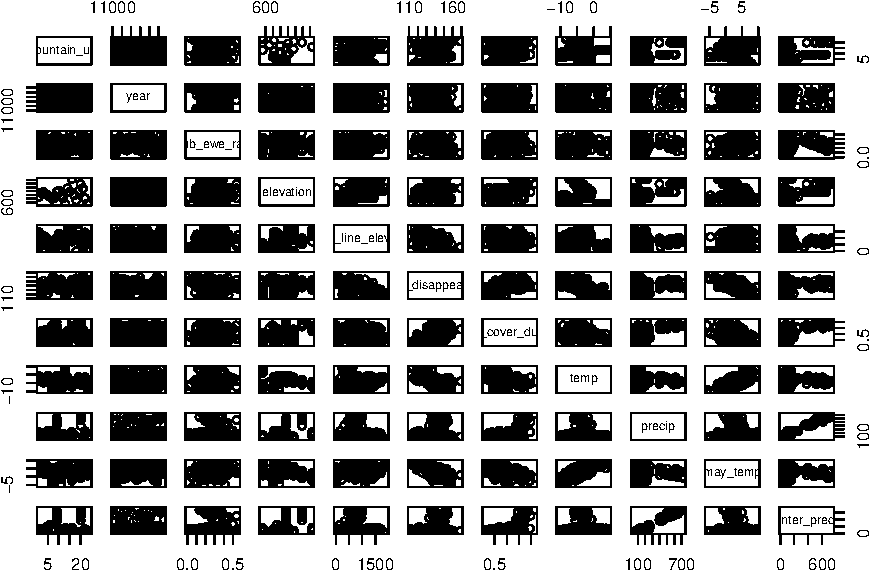
\includegraphics{FastFajardoPlasynski_ENV872_Project_files/figure-latex/unnamed-chunk-1-1.pdf}
\caption{Scatterplot matrix of dataset}
\end{figure}

\newpage

\begin{figure}
\centering
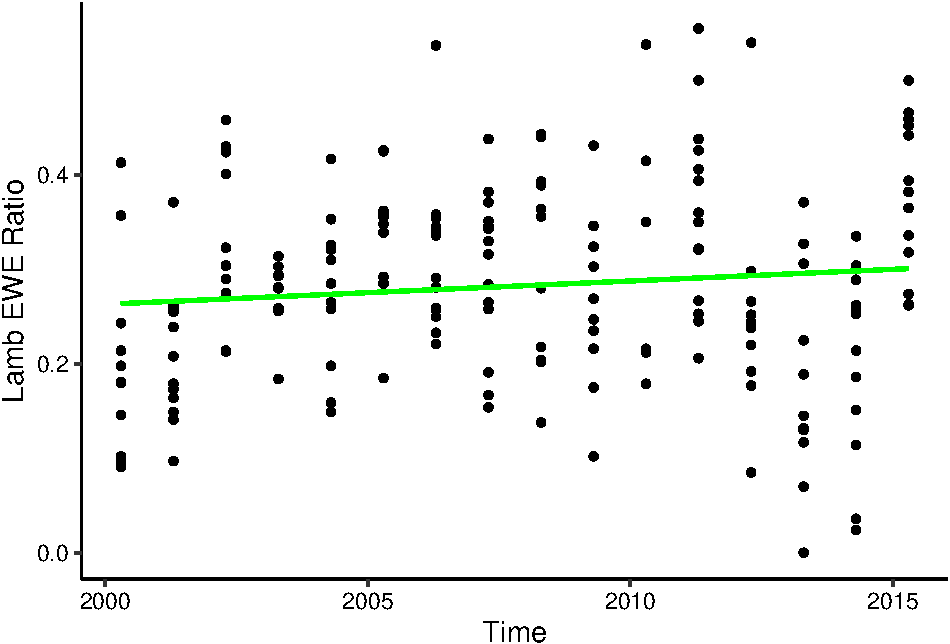
\includegraphics{FastFajardoPlasynski_ENV872_Project_files/figure-latex/unnamed-chunk-2-1.pdf}
\caption{Lamb EWE Ratio over Time}
\end{figure}

\begin{figure}
\centering
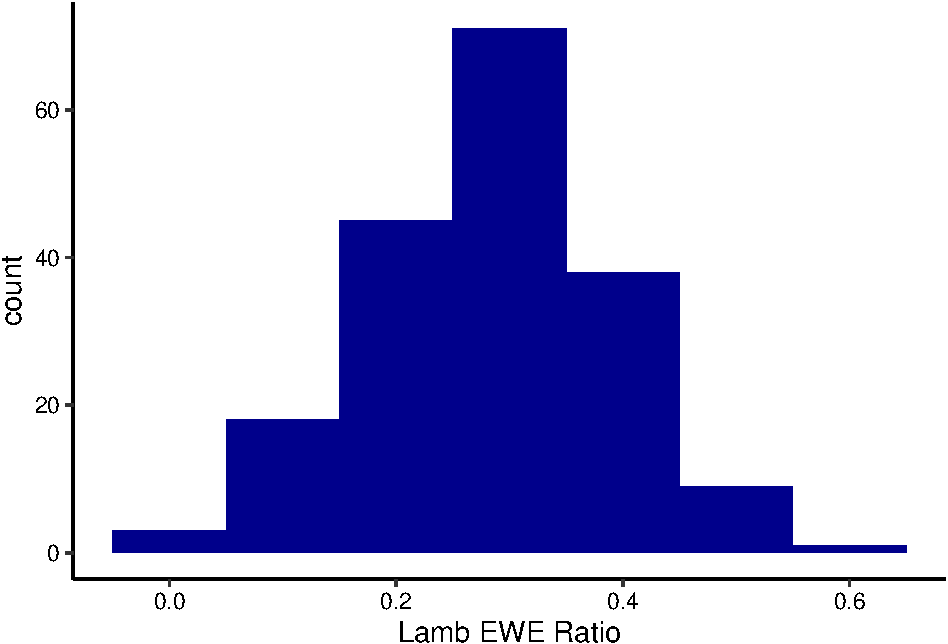
\includegraphics{FastFajardoPlasynski_ENV872_Project_files/figure-latex/unnamed-chunk-3-1.pdf}
\caption{Histogram of Lamb EWE Ratio}
\end{figure}

\begin{longtable}[]{@{}lrrrrrrrr@{}}
\caption{Summary Statistics of Lamb Dataset}\tabularnewline
\toprule
& vars & n & mean & sd & min & max & range & se \\
\midrule
\endfirsthead
\toprule
& vars & n & mean & sd & min & max & range & se \\
\midrule
\endhead
mountain\_unit & 1 & 185 & NaN & NA & Inf & -Inf & -Inf & NA \\
year & 2 & 185 & NaN & NA & Inf & -Inf & -Inf & NA \\
lamb\_ewe\_ratio & 3 & 185 & 0 & 0.107 & 0.000 & 0.555 & 0.555 &
0.008 \\
elevation & 4 & 185 & 1086 & 368.874 & 496.442 & 1852.819 & 1356.377 &
27.120 \\
snow\_line\_elevation & 5 & 185 & 800 & 486.914 & 0.000 & 1922.125 &
1922.125 & 35.799 \\
snow\_disappearance & 6 & 185 & 138 & 11.175 & 111.319 & 169.015 &
57.696 & 0.822 \\
snow\_cover\_duration & 7 & 185 & 1 & 0.091 & 0.417 & 0.830 & 0.413 &
0.007 \\
temp & 8 & 185 & -4 & 3.090 & -10.489 & 4.606 & 15.095 & 0.227 \\
precip & 9 & 185 & 189 & 169.379 & 30.743 & 725.153 & 694.410 &
12.453 \\
may\_temp & 10 & 185 & 3 & 2.975 & -5.690 & 9.779 & 15.469 & 0.219 \\
winter\_precip & 11 & 185 & 161 & 180.647 & 16.419 & 738.344 & 721.925 &
13.281 \\
\bottomrule
\end{longtable}

\begin{longtable}[]{@{}rrrr@{}}
\caption{Lamb EWE Ratio: Summary Table}\tabularnewline
\toprule
mean.ratio & minimum.ratio & maximum.ratio & sd.ratio \\
\midrule
\endfirsthead
\toprule
mean.ratio & minimum.ratio & maximum.ratio & sd.ratio \\
\midrule
\endhead
0.2825135 & 0 & 0.555 & 0.1067934 \\
\bottomrule
\end{longtable}

\newpage

\hypertarget{analysis}{%
\section{Analysis}\label{analysis}}

The best model, as chosen by AIC in a stepwise algorithm, included the
following explanatory variables: snow cover duration, temperature, and
May temperature. The final model indicates that about 7\% (adjusted
r-squared=0.06929) of the variation in the dependent variable is
explained by the independent variables. As indicated by the F-statistic,
the variables in the model are significantly different from 0,
demonstrating that the linear regression model fits the data better than
a model without any explanatory variables (Table 6).

The three explanatory variables were all statistically significant in
the final model, indicating that they have a statistically significant
effect on lamb ewe ratio. With a one unit increase in snow cover
duration, lamb ewe ratio increased by 0.293678 (snow cover duration:
estimate = 0.293678, p = 0.86777) (Table 6). This slight positive
relationship between lamb ewe ratio and snow cover duration is visible
in the plot, with the line of best fit sloping upwards (Figure 4).

With a one unit increase in temperature, lamb ewe ratio decreased by
0.013754 (temperature: estimate = -0.013754, p = 0.00140) (Table 6).
Given that this negative relationship between the two variables is very
slight, the line of best fit does not demonstrate this negative
relationship and instead appears to be a plateau (Figure 5).

With a one unit increase in May temperature, lamb ewe ratio increased by
0.020645 (May temperature: estimate = 0.020645, p = 6.79e-05) (Table 6).
This positive relationship between lamb ewe ratio and May temperature is
visible in the plot (Figure 6), with the line of best fit sloping
upwards. The relationship between these two variables is noticeably more
significant in this plot than for the plot comparing lamb ewe ratio and
snow cover duration (Figure 4).

After selecting the model, it was crucial to check whether it fit the
assumptions of a linear regression. The assumptions were checked using
the diagnostic plots of the final model (Figure 7). The first plot,
``Residuals vs Fitted'' is used to check whether there is a linear
relationship/linearity. As the red line does not severely depart from
the horizontal dotted line, this assumption is met. To determine whether
the residuals are normally distributed, the ``Normal Q-Q'' plot is
examined. This plot indicates that the residuals are normally
distributed as the points tend to follow the straight line. The
``Scale-Location'' plot is used to determine whether the model meets the
assumption of homoscedasticity (equal variance of residuals). As the
residuals are spread randomly along the horizontal line, the assumption
is fulfilled. Lastly, to check that there are no influential values in
the dataset, the ``Residuals vs Leverage'' plot is examined. While there
are some points that appear to be distanced from the majority of the
points, they do not fall outside Cook's distance - indicating that there
are no influential points.

\% Table created by stargazer v.5.2.3 by Marek Hlavac, Social Policy
Institute. E-mail: marek.hlavac at gmail.com \% Date and time: Wed, Apr
20, 2022 - 17:57:25

\begin{table}[!htbp] \centering 
  \caption{Linear Regression Results} 
  \label{} 
\begin{tabular}{@{\extracolsep{5pt}}lc} 
\\[-1.8ex]\hline 
\hline \\[-1.8ex] 
 & \multicolumn{1}{c}{\textit{Dependent variable:}} \\ 
\cline{2-2} 
\\[-1.8ex] & lamb\_ewe\_ratio \\ 
\hline \\[-1.8ex] 
 snow\_cover\_duration & 0.294$^{***}$ \\ 
  & (0.108) \\ 
  & \\ 
 temp & $-$0.014$^{***}$ \\ 
  & (0.004) \\ 
  & \\ 
 may\_temp & 0.021$^{***}$ \\ 
  & (0.005) \\ 
  & \\ 
 Constant & $-$0.014 \\ 
  & (0.086) \\ 
  & \\ 
\hline \\[-1.8ex] 
Observations & 185 \\ 
R$^{2}$ & 0.084 \\ 
Adjusted R$^{2}$ & 0.069 \\ 
Residual Std. Error & 0.103 (df = 181) \\ 
F Statistic & 5.566$^{***}$ (df = 3; 181) \\ 
\hline 
\hline \\[-1.8ex] 
\textit{Note:}  & \multicolumn{1}{r}{$^{*}$p$<$0.1; $^{**}$p$<$0.05; $^{***}$p$<$0.01} \\ 
\end{tabular} 
\end{table}

\begin{figure}
\centering
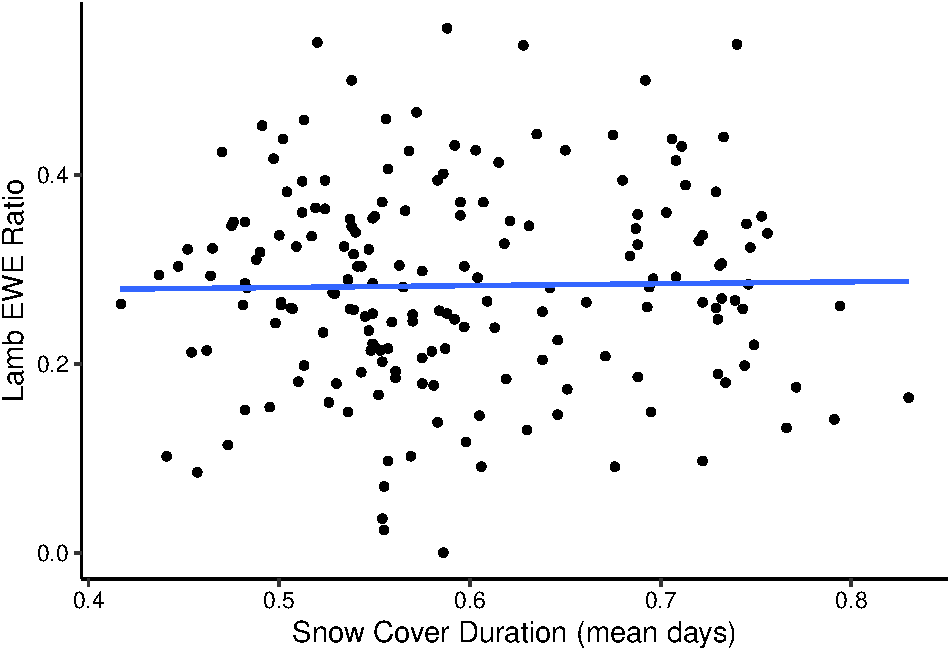
\includegraphics{FastFajardoPlasynski_ENV872_Project_files/figure-latex/unnamed-chunk-7-1.pdf}
\caption{Relationship between lamb EWE ratio and snow cover duration}
\end{figure}

\begin{figure}
\centering
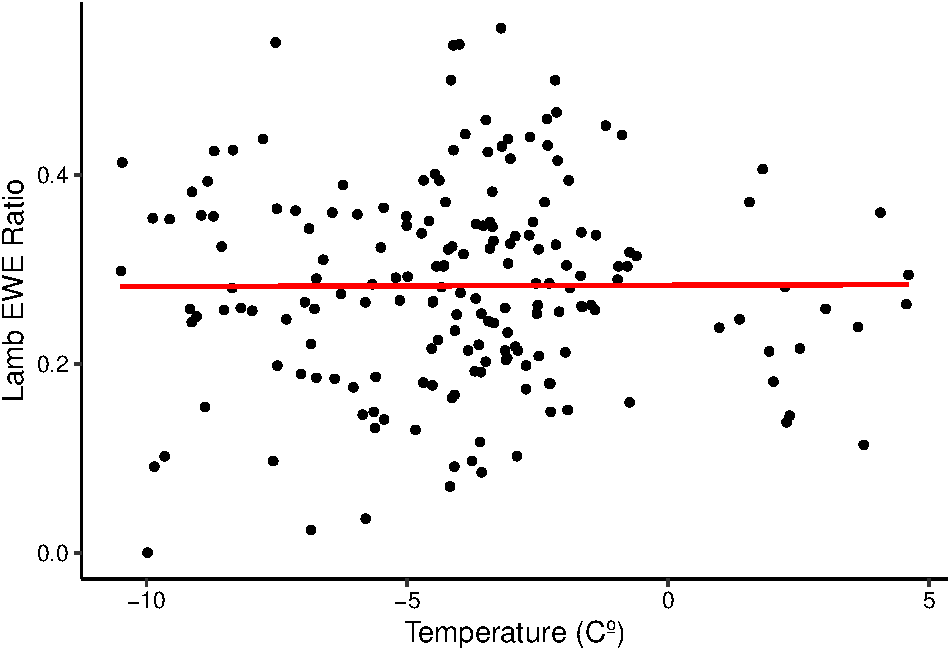
\includegraphics{FastFajardoPlasynski_ENV872_Project_files/figure-latex/unnamed-chunk-8-1.pdf}
\caption{Relationship between lamb EWE ratio and temperature (Cº)}
\end{figure}

\begin{figure}
\centering
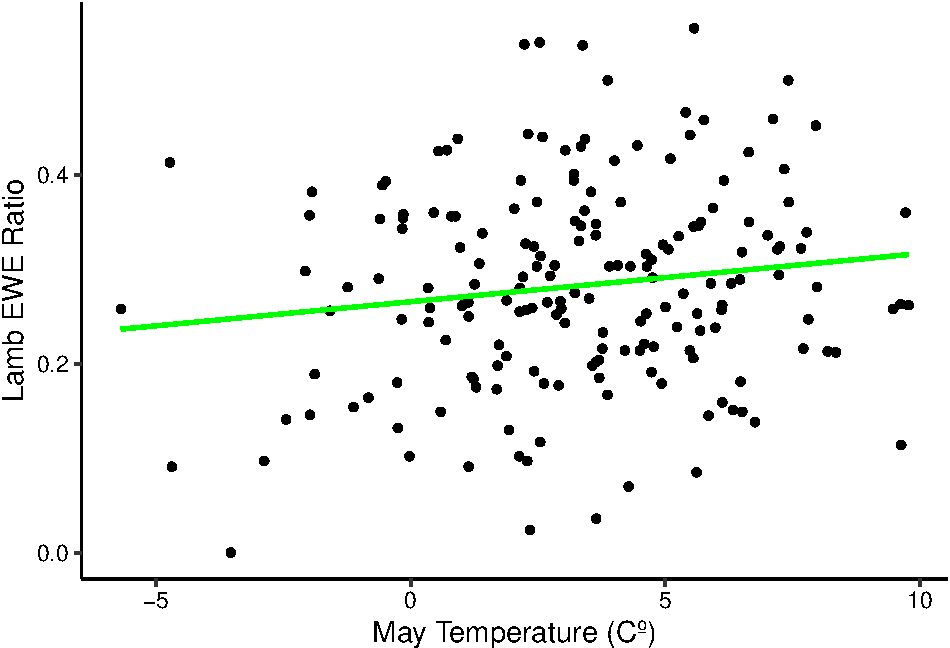
\includegraphics{FastFajardoPlasynski_ENV872_Project_files/figure-latex/unnamed-chunk-9-1.pdf}
\caption{Relationship between lamb EWE ratio and may temperature (Cº)}
\end{figure}

\begin{figure}
\centering
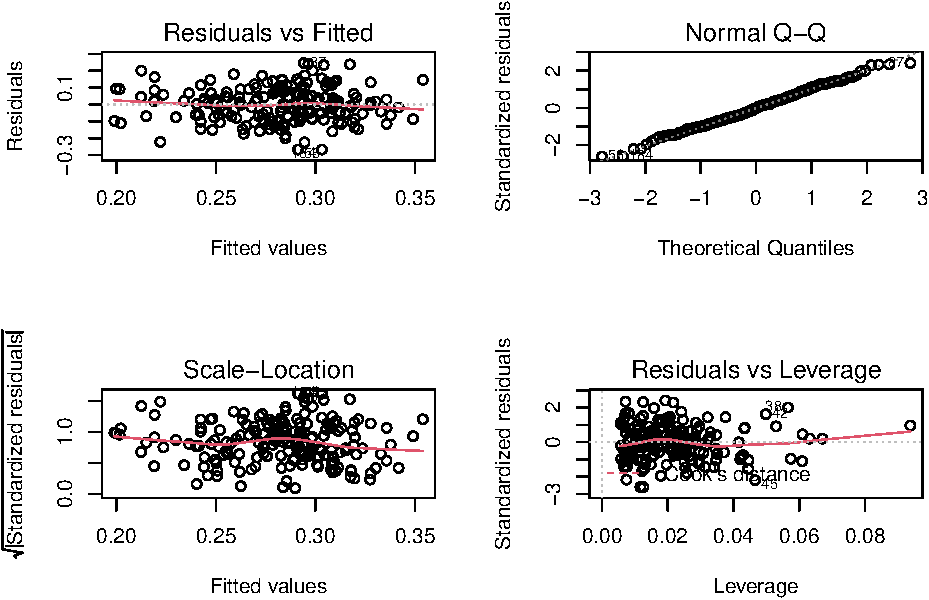
\includegraphics{FastFajardoPlasynski_ENV872_Project_files/figure-latex/unnamed-chunk-10-1.pdf}
\caption{Diagnostic plots of final model}
\end{figure}

\newpage

\hypertarget{summary-and-conclusions}{%
\section{Summary and Conclusions}\label{summary-and-conclusions}}

In summary, we found that some climatic conditions have a significant
effect on dall sheep reproductive success. Our results indicate that
reproductive success is reduced when overall temperatures are high,
likely due to adaptations of arctic species to thrive in colder
conditions with higher snow cover. This aligns with our findings that
reproductive success increases when snow cover duration is longer,
indicating again that colder overall temperatures benefit reproductive
success of dall sheep. Reproductive success also increased in response
to higher May temperature, indicating the importance of seasonal
temperature variation for population success. Survivability of offspring
likely depends heavily on seasonal vegetation, therefore high
temperatures in isolated months such as May are an important factor in
maintaining population stability.

Our results provide significant implications for future population
management. Arctic environments are experiencing increasing temperatures
at substantially higher rates than other areas, a trend that will also
contribute to decreased snow cover in Arctic North America (Corell,
2006). As climate change continues to affect environmental conditions,
we can expect dall sheep populations to decline in the future due to
evidence that increased temperatures and shorter snow cover duration
negatively impacts reproductive success. Because of this, it is
essential to form population management plans immediately to account for
the expected population decline and subsequent trophic cascade.
Management plans can include protected natural areas for these
populations, potentially at higher elevations and latitudes to
accommodate for migration to colder areas as temperatures rise.

\hypertarget{future-recommendations}{%
\section{Future Recommendations}\label{future-recommendations}}

For future research and analysis, more statistical tests should be
completed to look for interactions between variables. Additionally, more
data could be used in conjunction with this dataset to further analyze
our research question. Data on the rate of temperature and snow cover
duration change in Arctic North America can be used in conjunction with
this data set to estimate how heavily dall sheep reproductive success
will be affected in the future.

\newpage

\hypertarget{references}{%
\section{References}\label{references}}

Corell, R. W. (2006). Challenges of climate change: An arctic
perspective. AMBIO: A Journal of the Human Environment, 35(4), 148--152.
\url{https://doi.org/10.1579/0044-7447(2006)35\%5B148:coccaa\%5D2.0.co;2}

Higgins, M. E., \& Cassano, J. J. (2009). Impacts of reduced sea ice on
winter Arctic atmospheric circulation, precipitation, and temperature.
J. Geophys. Res., 114, D16107. \url{doi:10.1029/2009JD011884}

Kagata, H., \& Ohgushi, T. (2005). Bottom-up trophic cascades and
material transfer in Terrestrial Food Webs. Ecological Research, 21(1),
26--34. \url{https://doi.org/10.1007/s11284-005-0124-z}

Lambert Koizumi, C., \& Derocher, A. E. (2019). Predation risk and space
use of a declining dall sheep (ovis dalli dalli) population. PLOS ONE,
14(4). \url{https://doi.org/10.1371/journal.pone.0215519}

Post, E., \& Forchhammer, M. C. (2007). Climate change reduces
reproductive success of an Arctic herbivore through trophic mismatch.
Phil. Trans. R. Soc. B, 363(1501), 2367--2373.
\url{doi:10.1098/rstb.2007.2207}

\end{document}
